\chapter{Experimental Setups}
\label{chapter: Experimental Setups}

\par A small experimental setup using a simple object as a case study was built to prove the presented concepts and validate the design strategy. Moreover, this "proof of concept" experimental campaign was used to compare multiple optical configurations, assess their performance and investigate the underlying uncertainty sources. Later, a second experiment was conducted to improve the speckle pattern quality and image a compressible jet. All the information gathered was then applied to the visualization of the flow through an aerospike nozzle in a supersonic wind tunnel. The description of each setup follows below.

\par Each campaign is described by the same structure: the objective and the research question it addresses, the object of study, the optical layout and hardware, definition of the design points, the acquisition and processing settings, the sources of uncertainty specific to that setup, and the test matrix.


\section{Angled Glass Experiments}
\label{section: Angled Glass Experiment}

\par The first experimental campaign was envisioned to validate the surface maps presented in the last section and effectively compare a negative and positive defocus configuration in terms of its performance parameters for a similar object field of view. In order to achieve that, an experimental setup was built  where the optical distances could be easily set and modified. The setup was assembled on an optical rail close to the ground to avoid vibrations and followed the same structure as the schematic shown in Figure \ref{fig: SBOS with negative l}. 

\par Regarding hardware, Figure \ref{fig: Angled glass setup} shows the assembled setup. The laser used was a LIMAB model RC 0.5, a class 2 continuous red light laser ($\lambda = 632.8$ nm) with 0.5 mW of power. Given the class of the laser, safety was inherently guaranteed against accidental exposure, as the risk of eye injury is limited by the blink reflex. Nevertheless, simple procedures were made to make sure that the laser paths were contained and terminated. To diffuse the laser and create the speckle pattern, a small ground glass was used with only 1.27 cm of diameter. As it can be seen in the picture, the ground glass was positioned close to laser collimator, which was adjusted to fill the whole diameter of the ground glass. To image the displacements, LaVision's Imager sCMOS CLHS was used, it has a pixel size of 6.5 \si{\micro \meter} and a sensor dimension of $2560 \times 2160$ pixels. The camera was equipped mainly with a 200 mm camera lens. Two images with a 105 mm lens were taken, however, it was quickly changed back to the 200mm one, as it provided a more stable and robust assembly.

\begin{figure}[h]
    \centering
    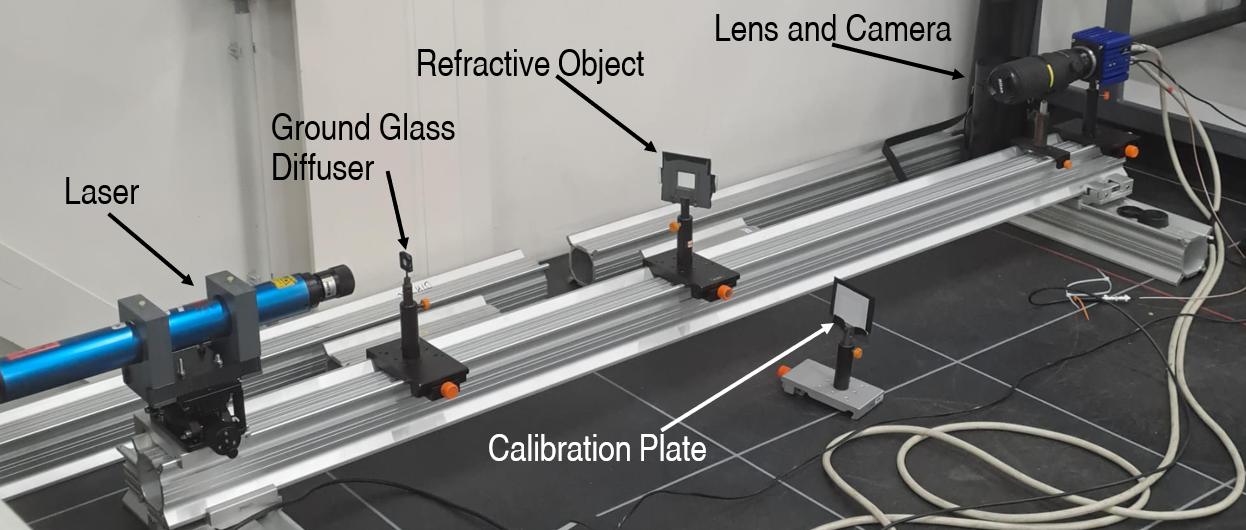
\includegraphics[width=\textwidth]{figures/small sbos setup with captions.png}
    \caption{Assembled setup of the angled glass campaign. The laser and the ground glass diffuser are mounted at the near end of the rail, the angled glass refractive object at mid-span and the lens and camera at the far end. The calibration plate, used to measure the optical magnification $M_{ag}$ in the in-focus plane, is shown on its own mount.}
    \label{fig: Angled glass setup}
\end{figure}



\par To simplify the experiment, a small angled piece of glass was used as refractive object, similar to what Schwarz \& Braukmann \cite{Schwarz&Braukmann} and Meier \& Rösgen \cite{Meier&Roesgen2013} have used. As shown in Figure \ref{fig: Angled glass geometry}, the angled glass introduces a uniform unidirectional displacement to the speckle background that can be predicted using Equation \ref{equation: Displacement of angled glass}. By dividing the displacement measured by the camera $\Delta x$ and the displacement induced by the refractive object $\varepsilon$, it is possible to obtain the setup sensitivity $S$, as shown in Equation \ref{equation: S BOS}. It is worth noting that the definition of $\varepsilon$ in this case is an artifice because the real displacement $\Delta x$ is independent of $l$. The $\varepsilon$ is used to connect a simple refractive object to a real experimental scenario. The glass piece used had a thickness $T = 2$ mm and a refractive index of around $n = 1.52 \pm 0.02$. 


 \begin{figure}[h]
   \centering
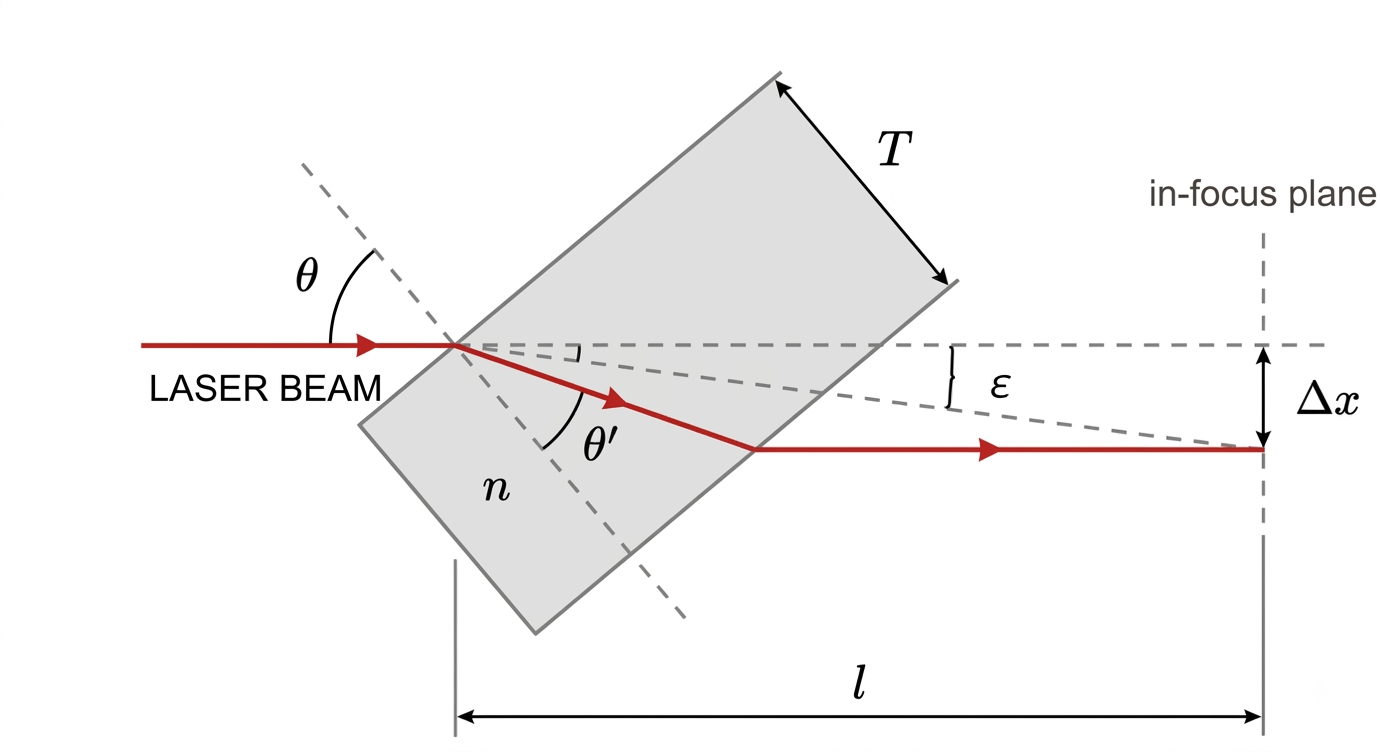
\includegraphics[width=0.7\textwidth]{figures/angled laser schematic.png}
    \caption{Geometry of the angled glass plate used as refractive object. A beam incident at an angle $\theta$ on a plate of thickness $T$ and refractive index $n$ is refracted to $\theta'$ and leaves the plate parallel to its original direction, laterally displaced by $\Delta x$. Over the defocus distance $l$ this displacement is equivalent to a uniform deflection angle $\varepsilon$.}
    \label{fig: Angled glass geometry}
\end{figure}

\begin{equation}
    \label{equation: Displacement of angled glass}
    \varepsilon = \frac{\Delta x}{l} =\frac{T}{l} \sin(\theta) \left( 1 - \frac{\cos(\theta)}{\sqrt{n^2-\sin^2(\theta)}}\right)
\end{equation}

\par Table \ref{tab: angled glass test matrix} shows the information of each point tested during the first campaign. The table lists not only the camera, lens configuration and optical distances, but also the theoretical magnification, sensitivity, predicted displacement given the measured glass angle and whether the in-focus plane was behind or in front of the refractive object. The points vary the type of configuration, the f-stop number, the defocus distance and the focal length of the camera and all of them have been obtained by computing the object field of view to be 2cm and inspecting the surface maps obtained with the code described in Chapter \ref{chapter: methodology}. In this instance then, the SR criterion has not been used, as the intention of the experiment was to validate the methodology by testing various different setups. Therefore, by comparing the theoretical sensitivity, magnification and the displacement with the ones obtained experimentally at each of these points, the methodology presented in Chapter \ref{chapter: methodology} can be validated. Moreover, through the comparison of experimental sensitivities obtained with a negative defocus against a positive defocus configuration, the difference in performance of SBOS versus BOS is obtained.

\begin{table}[h]
    \centering
    \caption{Optical configurations acquired during the angled glass campaign. $\theta$ is the angle at which the glass plate was set. ``Negative'' and ``Positive'' denote the in-focus plane lying respectively in front of or behind the test section, following the convention of Chapter \ref{chapter: methodology}. Points 1-9 correspond to the experiment with a similar $L_{FoV}$, whereas points 10-20 correspond to the linear slider experiment. In point 10 the refractive object is coincident with the in-focus plane, so no defocus type is defined.}
    \label{tab: angled glass test matrix}
    \begin{tabular}{lrrrrrrrl}
        \toprule
        Point & $f_\#$ & $f$ & $l$ & $d_f$ & $M_{ag}$ & $S$ & $\theta$  & Type of Defocus \\
              &         & [mm] & [mm] & [mm] & [--] & [mm] & [$^{\circ}$] & \\
        \midrule
        1    & 16 & 200 &  80 & 409.0 & 0.956 &  76.50 & 17 & Negative \\
        2    & 16 & 200 &  80 & 505.0 & 0.656 &  52.50 & 17  & Positive \\
        3    & 16 & 200 & 100 & 391.0 & 1.050 & 105.00 & 17  & Negative \\
        4    & 16 & 200 & 100 & 511.0 & 0.643 &  64.30 & 17  & Positive \\
        5   & 11 & 200 &  80 & 393.0 & 1.037 &  83.00 & 17  & Negative \\
        6   & 11 & 200 &  80 & 490.0 & 0.690 &  55.20 & 17  & Positive \\
        7   & 11 & 105 &  80 & 189.0 & 1.250 & 100.00 & 20  & Negative \\
        8   &  4 & 105 &  80 & 285.0 & 0.583 &  46.60 & 20  & Positive \\
        9   & 16 & 200 & 150 & 527.0 & 0.611 &  91.60 & 20  & Positive \\
        \midrule
        10 & 8 & 200 &  0 & 470.0 & 0.741 &  0.00 & 20    & --       \\
        11 & 8 & 200 & 10 & 470.0 & 0.741 &  7.41 & 20 & Positive \\
        12 & 8 & 200 & 20 & 470.0 & 0.741 & 14.81 & 20  & Positive \\
        13 & 8 & 200 & 30 & 470.0 & 0.741 & 22.22 & 20  & Positive \\
        14 & 8 & 200 & 40 & 470.0 & 0.741 & 29.63 & 20  & Positive \\
        15 & 8 & 200 & 50 & 470.0 & 0.741 & 37.04 & 20  & Positive \\
        16 & 8 & 200 & 10 & 470.0 & 0.741 &  7.41 & 20  & Negative \\
        17 & 8 & 200 & 20 & 470.0 & 0.741 & 14.81 & 20  & Negative \\
        18 & 8 & 200 & 30 & 470.0 & 0.741 & 22.22 & 20  & Negative \\
        19 & 8 & 200 & 40 & 470.0 & 0.741 & 29.63 & 20 & Negative \\
        20 & 8 & 200 & 50 & 470.0 & 0.741 & 37.04 & 20 & Negative \\
        \bottomrule
    \end{tabular}
\end{table}

Points 10-20 of Table \ref{tab: angled glass test matrix} describe the optical arrangement of a different configuration to the previous points. The setup presented in Figure \ref{fig: Angled glass setup} was modified to run an experiment intended to demonstrate the SBOS capacity of achieving different defocus configurations. The experiment consisted in keeping the in-focus plane fixed and moving the refractive object in steps with a linear slider, shown in Figure \ref{fig: Angled Glass Slider}. This kept the optical magnification constant, while permitting the exploration of a range of defocusing distances. Therefore the experiment can establish whether the advantage of the negative defocus configuration in achieving a higher sensitivity comes only from $M_{ag}$, or also from some other mechanism related to $l$.

The data acquisition followed standard BOS procedure using LaVision's DaVis 8.4 software. First, a calibration plate was used to define the in-focus plane, it can be seen in Figure \ref{fig: Angled glass setup}. From the calibration, DaVis computed the magnification and the pixel density of the setup. Then, the laser is turned on and a reference image is taken. The laser is turned back off and the refractive object is put into position following the distances presented in the surface maps of Chapter \ref{chapter: methodology}. With the laser back on, a displaced image is taken. Post-processing was done using LaVision DaVis 11 software. The images were first pre-processed to obtain a 2 frame sequence. Then the cross-correlation (CC) algorithm was used to reconstruct the displacement. Due to an unexpected large average speckle size, the smallest interrogation window had a size of $64 \times 64$ with 4 multipass and 75\% of overlap, while the biggest had $256 \times 256$ pixels with 1 pass and 75\% overlap. Nevertheless, given the large magnification, the vector pitch obtained is still quite small.


 \begin{figure}[h]
   \centering
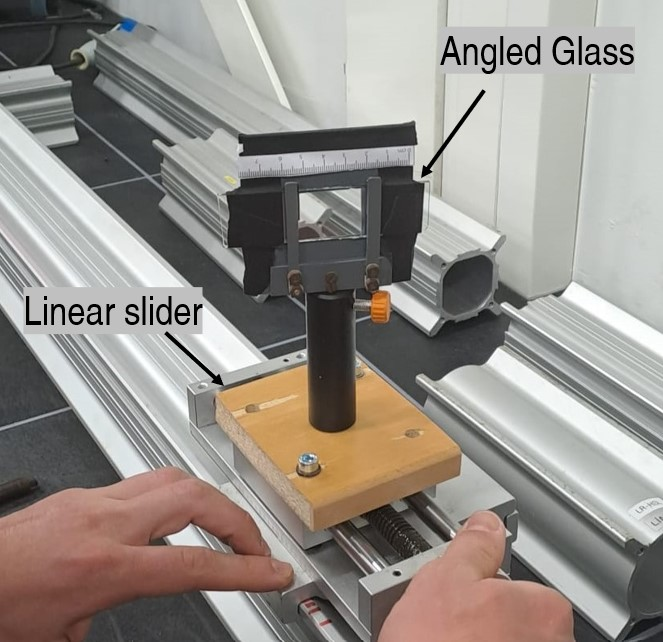
\includegraphics[width=0.5\textwidth]{figures/angled glass slider.jpeg}
    \caption{Picture of the angled glass in a linear slider, used to investigate the effect of $M_{ag}$ in the sensitivity}
    \label{fig: Angled Glass Slider}
\end{figure}

\subsection{Uncertainty Sources}
\label{subsection: angled glass uncertainty}

\par The campaign compares a displacement predicted by Equation \ref{equation: Displacement of angled glass} against a displacement measured by cross-correlation. Each side carries its own uncertainty, so two budgets are required before any disagreement between them can be interpreted. The defocus distance $l$ enters neither budget, since it cancels from the ratio of the predicted to the measured displacement. An error in $l$ can therefore not account for a disagreement between the two, although it does propagate into the sensitivity $S$.

\par Three quantities feed the prediction: the plate thickness $T$, the plate angle $\theta$ and the refractive index $n$. Thickness was measured with a calliper and the angle was set with a protractor. The refractive index was not measured and was taken from the value quoted for the glass, $n = 1.52 \pm 0.02$. Each input is treated as a rectangular distribution of half-width $a$, so its standard uncertainty is $u = a/\sqrt{3}$.

\par Sensitivity coefficients were obtained numerically from Equation \ref{equation: Displacement of angled glass} at both glass angles of the campaign. Table \ref{tab: angled glass uncertainty} collects them. The plate angle dominates. A deviation of $0.1^{\circ}$ moves the predicted displacement by 0.63\% at $\theta = 17^{\circ}$ and by 0.55\% at $\theta = 20^{\circ}$, whereas thickness and refractive index together account for less than half of the combined figure.

\begin{table}[h]
    \centering
    \caption{Uncertainty budget for the displacement predicted by Equation \ref{equation: Displacement of angled glass}. Each input is treated as a rectangular distribution of half-width $a$, so that $u = a/\sqrt{3}$. The last two columns give the relative contribution of each input to the predicted displacement at the two glass angles used in the campaign.}
    \label{tab: angled glass uncertainty}
    \begin{tabular}{llrrrr}
        \toprule
        Source & Instrument & $a$ & $u(x_i)$ & \multicolumn{2}{c}{Contribution [\%]} \\
        \cmidrule(lr){5-6}
               &            &     &          & $\theta = 17^{\circ}$ & $\theta = 20^{\circ}$ \\
        \midrule
        Plate thickness $T$  & Calliper   & 0.02 mm         & 0.012 mm         & 0.58 & 0.58 \\
        Refractive index $n$ & Literature & 0.02            & 0.012            & 1.40 & 1.37 \\
        Plate angle $\theta$ & Protractor & $0.50^{\circ}$  & $0.29^{\circ}$   & 1.82 & 1.59 \\
        \midrule
        Combined             &            &                 &                  & 2.37 & 2.18 \\
        \bottomrule
    \end{tabular}
\end{table}

\par Two quantities feed the measurement. The first is the scatter of the cross-correlation vector field $\sigma_\Delta$, already listed in Table \ref{tab: angled glass displacement results}, which runs from 2.0\% to 6.0\% of the mean displacement with an average of 3.2\%. The standard deviation of the field is used here in place of the standard error of the mean, because a 75\% window overlap leaves neighbouring vectors strongly correlated and the effective number of independent samples well below the vector count. The second is the optical magnification returned by the DaVis calibration, which converts the measured displacement from pixels to millimetres. \todo{insert the DaVis calibration fit residual}

\par The two budgets combine in quadrature to a standard uncertainty of approximately 4\% on the comparison between prediction and measurement, or 8\% at a coverage factor of $k = 2$. \todo{recompute once the calibration residual is available}

\par Three consequences follow for the results of Chapter \ref{chapter: Results}. Points 2 to 9 disagree by 0.5\% to 2.6\%, which falls below the standard uncertainty and calls for no further explanation. Point 1 shows the largest disagreement of the campaign at 7.9\%, close to twice the standard uncertainty and at the edge of the interval defined by $k = 2$. The value stays compatible with the budget as a whole, although no single input accounts for it on its own: an error in $\theta$ alone would have to reach $1.26^{\circ}$, which exceeds the reading uncertainty of the protractor by more than a factor of four. Points 10 to 20 sit between 2.4\% and 3.7\%, all of the same sign and with no dependence on $l$. A one-signed offset of this kind indicates a systematic error rather than scatter, and an angle offset of $0.57^{\circ}$ reproduces it exactly. Those eleven points share a single setting of the glass plate, so a small constant error in $\theta$ is the most plausible source.

\par No beam expander was used during the first experimental campaign. Since no specification in the literature was found to size the laser diffuser and given the small field of view of 2cm, it was believed that the scattering and diffusion alone from the ground glass would be sufficient to fill the whole field of view. However that belief was proven wrong. Moreover, the small size of the diffuser made the laser beam diffraction limited at the ground glass and not at the camera aperture, this meant that changing the f-stop of the camera had no effect in the average speckle pattern size and the average speckles were a lot bigger than expected. Another effect was the vignetting of the speckle pattern diameter, meaning that the pattern size would change with the aperture diameter and magnification ($D_{\Delta s} \approx D \cdot M_{ag}$), which limited the usable $f_\#$. Faced with these limitations, another experimental campaign was envisioned with a bigger ground glass and a beam expander to try and produce a finer speckle pattern.

\section{Speckle Pattern Investigation}
\label{section: Speckle Pattern Investigation}
The second experimental campaign was intended to investigate further the speckle pattern and tackle the limitations of the first experiments. The main goals were to better understand the creation of a finer speckle pattern that would not experience vignetting, assess how the average speckle size correlates to the Rayleigh limit of Equation \ref{equation: Rayleigh Limit} and also compare the generation of speckles through direct ground glass diffusion and by projecting the laser into a surface. The setup used for the direct speckles investigation resembles the one shown in Section \ref{section: Angled Glass Experiment} and can be seen in Figure \ref{fig: Directed speckles investigation setup}.

\begin{figure}[h]
    \centering
    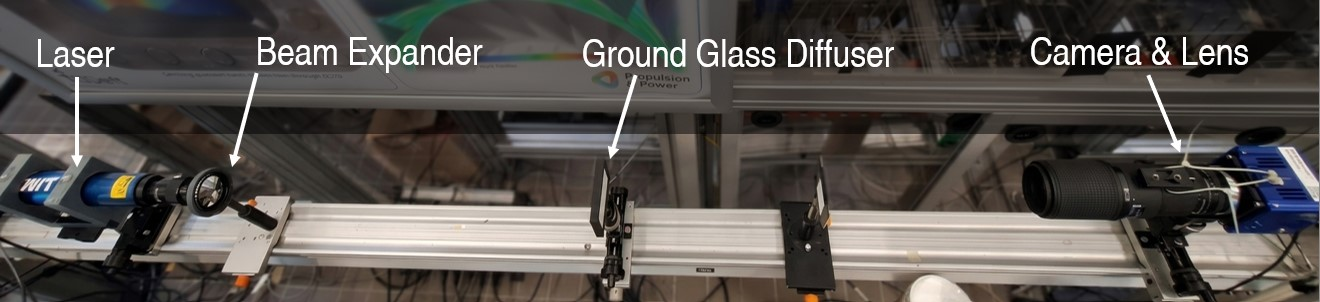
\includegraphics[width=\textwidth]{figures/speckle pattern investigation.jpg}
    \caption{Assembled directed speckle investigation setup. Configuration is quite similar from the one presented in Section \ref{section: Angled Glass Experiment} with the distinct presence of the beam expander lens in-between the laser and ground glass diffuser.}
    \label{fig: Directed speckles investigation setup}
\end{figure}

%%Modify this Picture ^^^ to show dgg and df

The main difference between the setup in Figure \ref{fig: Angled glass setup} and the one in Figure \ref{fig: Directed speckles investigation setup} is the presence of a larger ground glass diffuser and a lens to expand the laser beam. The new ground glass diffuser has 88 mm of length and 61 mm of width, which makes it capable of filling larger fields of view. The beam expander consists of a convergent lens with focal length of $f = 80$ mm, positioned at a distance $d_{GG}$ behind the ground glass, which was varied to see its effects in the speckle creation. The camera and laser are the same from the last experiment, only the camera lens with $f=200$mm was used.

A series of pictures were taken where $d_{GG}, M_{ag}$ and $f_\#$ were varied. Table \ref{tab: speckle investigation matrix} summarizes the experimental condition of each picture. The average speckle size was then computed using LaVision's DaVis 11 software processing function \emph{particle/speckle size over time} which computes the spatial averaged particle size through a defined sliding average length and subtracting the sliding minimum \cite{Pan2010}. For this application, both quantities were set to 16 pixels. These pictures will enable the selection of a ground glass distance capable of producing the desired speckle pattern, it will also quantify the effect of the magnification and f-stop number in the speckle production.

\begin{table}[h]
    \centering
    \caption{Configurations acquired during the speckle pattern investigation.
    $d_{GG}$ is the distance between the beam expander lens and the ground glass
    diffuser, $M_{ag}$ the magnification measured from the calibration and
    $\Delta s_{th}$ the speckle size predicted by the Rayleigh criterion
    (Equation \ref{equation: Rayleigh Limit}).}
    \label{tab: speckle investigation matrix}
    \begin{tabular}{lrrrrr}
        \toprule
        Point & $f_\#$ & $d_{GG}$ & $M_{ag}$ & $d_f$ & $\Delta s_{th}$ \\
              &         & [mm]     & [--] & [mm] & [px] \\
        \midrule
         1 &  4 & 740 & 0.9635 & 415 & 0.93 \\
         2 & 11 & 740 & 0.9635 & 415 & 2.57 \\
         3 & 22 & 740 & 0.9635 & 415 & 5.13 \\
         4 &  4 & 740 & 0.2956 & 930 & 0.62 \\
         5 & 11 & 740 & 0.2956 & 930 & 1.69 \\
         6 & 22 & 740 & 0.2956 & 930 & 3.39 \\
         7 & 11 & 450 & 0.2956 & 930 & 1.69 \\
         8 & 11 & 280 & 0.2956 & 930 & 1.69 \\
         9 & 11 & 190 & 0.2956 & 930 & 1.69 \\
        10 & 11 & 100 & 0.2956 & 930 & 1.69 \\
        11 &  4 & 300 & 0.4572 & 680 & 0.69 \\
        12 & 11 & 300 & 0.4572 & 680 & 1.90 \\
        13 & 22 & 300 & 0.4572 & 680 & 3.81 \\
        \bottomrule
    \end{tabular}
\end{table}

% This table is missing the experiments where we varied the zoom based on the lens indications, worth adding here (??) Definitely.

\begin{figure}[h]
    \centering
    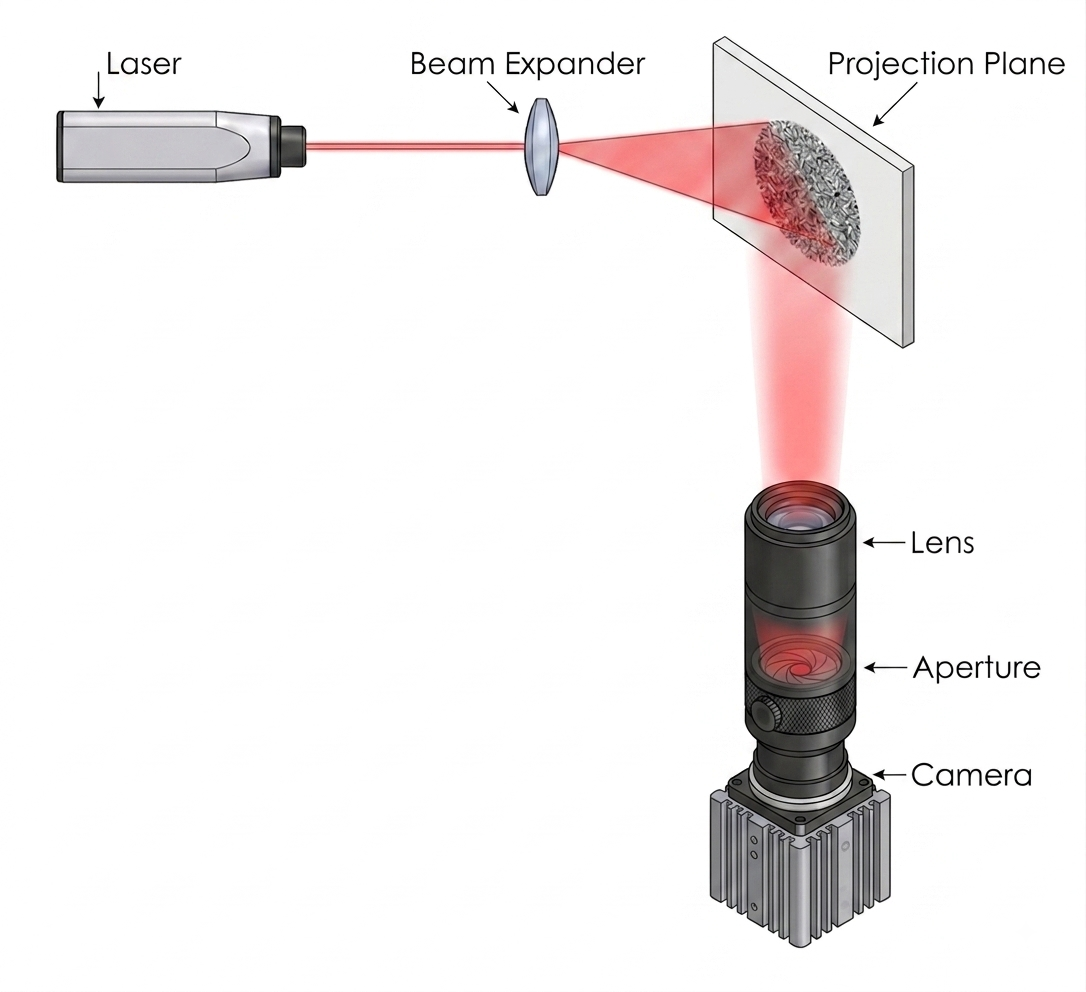
\includegraphics[width=0.5\textwidth]{figures/projected speckle schematic.png}
    \caption{Diagram of the setup used to create and study projected speckles}
    \label{fig: projected speckle setup diagram}
\end{figure}

The previous setup was modified to also test the creation of speckles by projecting the laser in a blank canvas, similar to what was done by Meier \& Rösgen and Bühlmann \cite{Meier&Roesgen2013,Buhlmann2020}. As shown by the schematic in Figure \ref{fig: projected speckle setup diagram}, a blank surface angled at $45^{\circ}$ has been placed in the beam path and the camera assembly has been moved to a perpendicular beam. The laser is expanded by the same $f=80$ mm lens. When it hits the surface, its light diffuses and creates an interference pattern captured by the camera. Figure \ref{fig: projected speckle experiment} shows a picture of the speckle pattern being generated in the projection plane, there it is also possible to see the camera assembly and the beam expander.


\begin{figure}[h]
    \centering
    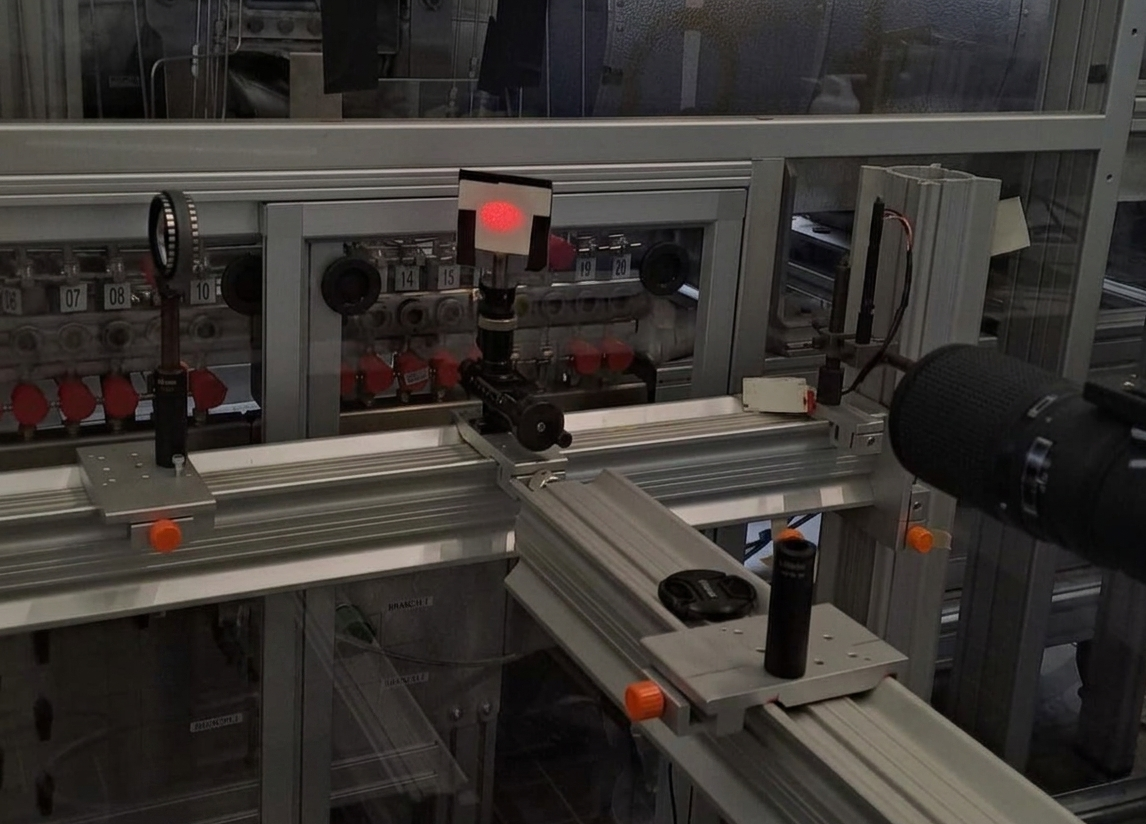
\includegraphics[width=0.7\textwidth]{figures/projected speckle pattern experiment.png}
    \caption{Photograph of the projected speckle experimental setup. In the projection plane it is possible to see the speckle pattern formed}
    \label{fig: projected speckle experiment}
\end{figure}

\subsection{Uncertainty Sources}
\label{subsection: speckle uncertainty}

\par This campaign sets a measured average speckle size against the Rayleigh limit of Equation \ref{equation: Rayleigh Limit}. The two quantities are not equivalent. Equation \ref{equation: Rayleigh Limit} returns the smallest speckle the optical system can form, whereas the DaVis function returns a spatial average over a real pattern. A measured value above the prediction is therefore the expected outcome, and the comparison tests a floor rather than an equality. Only a measured value below the limit would indicate an error.

\par The prediction rests on three inputs. The wavelength is fixed by the laser line at $\lambda = 632.8$ nm and contributes nothing of consequence. The optical magnification comes from the same DaVis calibration discussed in Subsection \ref{subsection: angled glass uncertainty}, so its uncertainty carries over unchanged. The f-stop number deserves attention, because the values engraved on a lens barrel are rounded members of a geometric series. Table \ref{tab: fstop correction} lists the effect. Marked apertures of 4, 8 and 16 are exact, whereas 11 and 22 stand for 11.31 and 22.63. The $\Delta s_{th}$ column of Table \ref{tab: speckle investigation matrix} is consequently low by 2.9\% for the ten points acquired at those two settings.

\begin{table}[h]
    \centering
    \caption{Effect of the rounded f-stop scale on the speckle size predicted by Equation \ref{equation: Rayleigh Limit}. The engraved values follow powers of $\sqrt{2}$, and two of the three settings of this campaign are rounded. The correction applies to every point of Table \ref{tab: speckle investigation matrix} acquired at $f_\# = 11$ or $f_\# = 22$.}
    \label{tab: fstop correction}
    \begin{tabular}{lrrl}
        \toprule
        Marked $f_\#$ & Actual $f_\#$ & Correction on $\Delta s_{th}$ & Points affected \\
        \midrule
        4  &  4.00 & 0.0\% & 1, 4, 11 \\
        11 & 11.31 & 2.9\% & 2, 5, 7, 8, 9, 10, 12 \\
        22 & 22.63 & 2.9\% & 3, 6, 13 \\
        \bottomrule
    \end{tabular}
\end{table}

\par On the measurement side the dominant term is the estimator itself. The DaVis function subtracts a sliding minimum from a sliding average, and both lengths were fixed at 16 pixels for every point of the campaign. That choice is arbitrary and the returned size depends on it. A repeat of the analysis at other lengths bounds the effect. \todo{repeat the speckle size analysis at 8 and 32 px and quote the spread}

\par Speckle formation is random in nature, as established in Chapter \ref{chapter: LiteratureReview}. A single image therefore yields a finite sample estimate rather than a fixed property of the setup, and the spread across the field or across repeated frames sets a statistical floor that no choice of estimator can improve upon. \todo{quote the standard deviation of the speckle size across the field}

\par One condition governs whether the comparison is meaningful at all. Section \ref{section: Angled Glass Experiment} established that the small diffuser of the first campaign made the beam diffraction limited at the ground glass instead of at the camera aperture, which placed the setup outside the regime that Equation \ref{equation: Rayleigh Limit} describes. The larger diffuser was introduced to restore that regime. Evidence for the restoration is the response of the measured size to the f-stop, since a diffraction limit set at the aperture must scale with $f_\#$ and one set at the diffuser must not. Points 1 to 3, 4 to 6 and 11 to 13 each hold the magnification fixed and vary only the aperture, so the three groups provide that test directly. Residual vignetting would break the same condition across the field and is checked by a comparison of the estimate between the centre and the edge of the image.

Up until now, the designed setup made it known how to create an appropriate speckle pattern and how to set the optical distances so a desirable sensitivity and spatial resolution is achieved. This knowledge now can be applied in a proof of concept case that enables the visualization of a true density gradient and even its integration into a density field. The next experiment will build on that basis to visualize a compressible jet, which will serve as proof of concept and allow for the reconstruction of a density field using SBOS.

\section{Compressible Jet Experiment}
\label{section: Compressible jet experiment}

A similar setup to the one shown in Figure \ref{fig: Directed speckles investigation setup} was used to image a compressible jet. For this experiment, $l = 3$ cm, $d_{GG} = 83$ cm, $d_f = 74$ cm and $f_\# = 11$, which gives $M_{ag} = 0.37$, $S = 11.1$ mm and $s_{min} = 0.369$ mm. Figure \ref{fig: Compressible Jet experiment} shows a picture of the assembled setup. The jet was achieved by connecting a standard air gun with a nozzle diameter $d_N = 3.5$ mm to a wall air tap with a hose. This setup allowed to adjust the pressure coming out of the air tap, however, a big limitation was the lack of loss quantification through the hose, quick-disconnect couplings and the air gun itself, meaning that the actual pressure right before the nozzle exit was unknown.

\begin{figure}[h]
    \centering
    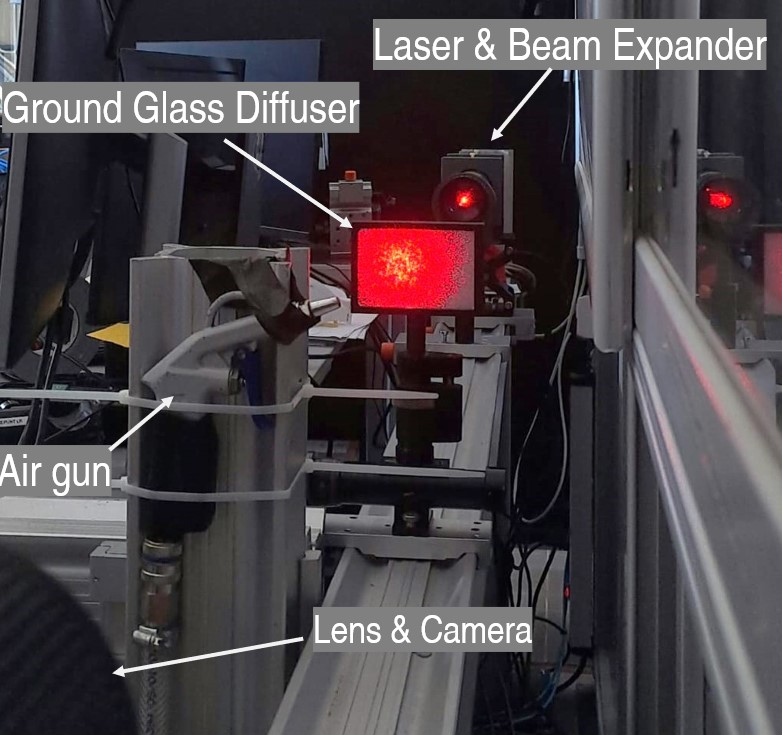
\includegraphics[width=0.5\textwidth]{figures/compressible jet setup.jpeg}
    \caption{Photograph of the compressible jet experimental setup.}
    \label{fig: Compressible Jet experiment}
\end{figure}

The data acquisition followed a similar procedure than the one explained at Section \ref{section: Angled Glass Experiment}. A target plate was put at the in-focus position and a picture was captured to calibrate laVision's DaVis software. Then, the laser was turned on and a reference picture was taken. The pressure was set at the air tap valve and the air gun was triggered, while the camera captured 100 images with an exposure time of 300 $\mu$s. In total, 6 cases were captured with pressures at the air tap valve ranging from 3 bar to 8 bar with 1 bar step. The speckle size obtained was checked following the procedure of Section \ref{section: Speckle Pattern Investigation}. The 100 images for each case were averaged and cross-correlated with an interrogation window of 12 px, 75\% of overlap and 4 multipasses.


\subsection{Uncertainty Sources}
\label{subsection: jet uncertainty}

\par The jet measurement runs through a longer chain than the two campaigns before it. A displacement field is converted into a deflection angle, the deflection angle into a density gradient through the Gladstone-Dale relation, and the gradient into a density field through the inverse Abel transform of Subsection \ref{subsection: Axisymmetric Refractive Field}. Every stage adds a term, and the terms fall into three groups: the flow condition, the optical setup, and the reconstruction.

\par The flow condition carries the largest uncertainty and the one least under control. As stated at the start of this section, the pressure at the air tap valve is known but the pressure immediately upstream of the nozzle is not, because the losses across the hose, the quick-disconnect couplings and the air gun body were never quantified. Any comparison against compressible flow theory inherits that gap, since the nozzle pressure ratio follows from the stagnation pressure alone. An independent route exists. The shock cell length of an underexpanded jet depends on the nozzle pressure ratio through the relation of Emden \cite{Emden1899}, so a measurement of the cell length recovers the pressure without a gauge at the nozzle. \todo{bound the nozzle pressure from the measured shock cell length}

\par The optical terms are those of Subsection \ref{subsection: angled glass uncertainty} and transfer without modification. Sensitivity follows from $S = l M_{ag}$, so the defocus distance and the calibration magnification enter directly. Both were set once for the whole pressure series, which makes their contribution a common bias across the six cases rather than a source of scatter between them. Relative comparisons between pressures are therefore tighter than the absolute density level.

\par Processing contributes a term that the current settings hide. The 100 frames of each case were averaged before cross-correlation, so the algorithm returns a single mean field and no estimate of its own repeatability. Correlation of the frames individually recovers that estimate, and the standard deviation across the 100 realisations then plays the role that $\sigma_\Delta$ plays in Table \ref{tab: angled glass displacement results}. The same operation separates measurement noise from genuine unsteadiness in the jet, which the average discards. \todo{correlate the frames individually and quote the scatter across realisations}

\par Three terms belong to the reconstruction. The Gladstone-Dale coefficient for air at $\lambda = 632.8$ nm is known to better than one percent and is negligible against the rest. The width assigned to the refractive object in the near-field correction is not measured but inferred, so its influence on the recovered density needs a sensitivity study across a plausible range. \todo{quantify the density sensitivity to the assumed object width} The inverse Abel transform assumes axial symmetry and involves a derivative, which amplifies noise towards the jet axis and makes the centreline density the least reliable part of the field. A jet from a commercial air gun nozzle is unlikely to be perfectly symmetric, and a comparison of the two halves of the measured field quantifies the departure.

\section{Aerospike Experiment}